\documentclass[11pt,a4paper]{article}
\usepackage[T1]{fontenc}
\usepackage[utf8]{inputenc}
\usepackage{lmodern,amsmath,amssymb,amsthm,booktabs,array,graphicx,float}
\usepackage[margin=25mm]{geometry}
\usepackage[dvipsnames]{xcolor}
\usepackage[colorlinks=true,linkcolor=MidnightBlue,citecolor=MidnightBlue,urlcolor=MidnightBlue]{hyperref}
\usepackage{microtype}
\newtheorem{theorem}{Theorem}[section]
\newtheorem{lemma}[theorem]{Lemma}
\newtheorem{corollary}[theorem]{Corollary}
\theoremstyle{remark}
\newtheorem{remark}[theorem]{Remark}
\newcommand{\norm}[1]{\left\lVert#1\right\rVert}
\newcommand{\tr}{\operatorname{tr}}
\newcommand{\STAB}{\operatorname{STAB}}
\newcommand{\MATCH}{\operatorname{MATCH}}
\newcommand{\BETA}{\operatorname{BETA}}
\newcommand{\R}{\mathbb R}
\setlength{\emergencystretch}{2em}
\setlength{\parskip}{3pt}

\title{Exact weighted Pauli uncertainty on line graphs via the matching polytope\thanks{Independent
working manuscript. Author metadata and disclosure statement must be completed
before submission.}}
\author{Anonymous author\\Independent researcher}
\date{17 September 2026}

\begin{document}
\maketitle

\begin{abstract}
For Pauli observables, let the frustration graph join exactly the
anticommuting pairs. We prove that the complete weighted quadratic uncertainty
problem is exact on every line graph. For every finite simple graph $R$, the
representation-independent beta body is exactly the matching polytope,
\[
 \BETA(L(R))=\MATCH(R).
\]
Equivalently, for every nonnegative edge weight $w$,
\[
 \beta(L(R),w)=\alpha(L(R),w)=\nu(R,w),
\]
where $\nu(R,w)$ is the maximum weight of a matching of $R$. The main proof
maps the Hamiltonian to a Majorana bilinear. Nuclear-norm duality produces
a skew contraction $Q$, and the squared supported entries $Q_e^2$ satisfy
both the degree and all odd-set inequalities of Edmonds' matching polytope.
It also yields the sharp matrix inequality
\[
 \left(\norm{A}_*/2\right)^2\leq
 \nu(R,w)\sum_{e\in E(R)}A_e^2/w_e
\]
for every real skew matrix supported on $R$. The family $L(K_{2k+1})$,
$k\geq2$, proves that the theorem strictly extends the previously sufficient
$h$-perfect route. An exhaustive small-root ablation separates the mechanism:
degree constraints are exact on 66.89\% of 6225 weighted instances, cliques
plus odd cycles on 84.69\%, and the complete odd-set system on 100\%. Removing
skewness fails already on a triangle. As a secondary extension, we prove that
every simplicial claw-free quasi-line graph is rank-perfect and hence
$\hbar$-perfect. The analytic theorem, not the finite computation, carries the
claim.
\end{abstract}

\noindent\textbf{Status and scope.}
This is a self-contained working manuscript, not an externally reviewed
article. The proof uses classical matching-polytope and Majorana tools, which
are cited explicitly. A documented search found no prior statement of the
body identity or all-weight equality above, but a negative literature search
is not a proof of priority. The expanded C045 search was frozen on 16 September
2026 and found no exact collision, but this remains support rather than
certification. A C046 mock-referee pass formalized the body-level statement and
audited every dependency in the central proof.
No quantum advantage or new matching algorithm is claimed.

\section{Introduction}

Let $P_1,\ldots,P_n$ be Hermitian Pauli observables. Their frustration graph
$G$ has vertex set $[n]$ and an edge $ij$ exactly when
$P_iP_j=-P_jP_i$; nonedges commute. For nonnegative $w$, define
\begin{equation}\label{eq:beta}
 \beta(G,w)=\max_\rho\sum_i w_i\tr(\rho P_i)^2,
 \qquad
 \alpha(G,w)=\max_{S\text{ stable in }G}\sum_{i\in S}w_i.
\end{equation}
Here the first maximum may use any Pauli realization with exactly the
prescribed pairwise relations: its value is representation-independent by the
beta-number framework of Xu et al.~\cite{xu,xuprx}. Since the observables in
a stable set commute, a common eigenstate gives
$\beta(G,w)\geq\alpha(G,w)$. The difficult direction is the upper bound.

The equality $\beta(G,w)=\alpha(G,w)$ for every nonnegative $w$ is called
$\hbar$-perfection~\cite{xu}. Known sufficient classes do not settle all line
graphs. Line graphs are also the natural frustration graphs of quadratic
Majorana Hamiltonians~\cite{cf,cem}, while their stable sets are precisely
matchings. This suggests that a quantum uncertainty body and a classical
matching polytope might coincide. The missing issue is not the degree
constraints but the entire family of blossom, or odd-set, constraints.

Our contribution is a direct mechanism for all of them. If $Q$ is a skew
contraction, every odd principal submatrix loses at least one rank. This turns
its Frobenius norm into the corresponding odd-set inequality. Together with
row-norm degree constraints, Edmonds' theorem identifies the squared entries
of $Q$ as a point of the matching polytope. Weighted Cauchy--Schwarz then
closes the quantum bound exactly.

The resulting theorem has three useful forms:
\begin{enumerate}
 \item every finite line graph is $\hbar$-perfect;
 \item every nonnegative weighted instance is solved by maximum-weight
 matching, without state simulation;
 \item a sharp support-sensitive nuclear-norm inequality holds for all real
 skew matrices.
\end{enumerate}
The last form distinguishes the result from a merely unweighted skew-energy
estimate. We also give an independent proof through known simplicial
claw-free rank bounds and exhibit an infinite separation from the
$h$-perfect sufficient class. Finally, rather than reporting only successful
theorem checks, we compare the complete mechanism against two explicit weaker
baselines and ablate skewness itself.
As a secondary extension, we combine a simplicial-clique heredity lemma with
the modern facet structure of fuzzy circular interval graphs to prove
$\hbar$-perfection for simplicial claw-free quasi-line graphs. This extension
is separated from the headline contribution because it depends on the
classical quasi-line facet classification.

\section{Definitions and the variational reduction}

For a fixed Pauli realization $\mathcal S=\{P_i\}_{i\in V(G)}$, write
\[
 \mathcal Q(\mathcal S)=
 \left\{\bigl(\tr(\rho P_i)^2\bigr)_{i\in V(G)}:\rho\text{ a state}\right\}.
\]
If $T\subseteq\R^{V(G)}$, let
$\mathord\downarrow T=\{x:\text{ there is }y\in T\text{ with }0\leq x\leq y\}$.
Proposition~1 of Xu et al.~\cite{xu} proves that
\begin{equation}\label{eq:beta-body}
 \BETA(G)=\operatorname{conv}(\mathord\downarrow\mathcal Q(\mathcal S))
 \quad\text{and}\quad
 \beta(G,w)=\max_{y\in\BETA(G)}w\mathbin{\cdot}y
 \quad(w\geq0)
\end{equation}
are independent of the chosen realization. Thus $\BETA(G)$ is a compact
convex corner, whereas the raw joint range $\mathcal Q(\mathcal S)$ need not be
convex and can depend on the realization. This distinction is essential for
the body-level statement below.

For a finite simple root graph $R=(V,E)$, its line graph $L(R)$ has one vertex
for every edge of $R$; two vertices are adjacent when their root edges share
an endpoint. A matching of $R$ is therefore a stable set of $L(R)$, and
\begin{equation}\label{eq:alpha-nu}
 \alpha(L(R),w)=\nu(R,w),
\end{equation}
where $\nu(R,w)$ denotes maximum matching weight.

We use the following elementary variational identity. For fixed observables,
\begin{equation}\label{eq:variational}
 \max_\rho\sum_i w_i\tr(\rho P_i)^2
 =\max_{\norm{a}_2=1}\norm{\sum_i a_i\sqrt{w_i}P_i}^2.
\end{equation}
Indeed, Euclidean duality rewrites the squared norm of the expectation vector
as a maximization over $a$. For fixed $a$, maximization over density matrices
gives the squared spectral norm of the Hermitian linear combination. Compactness
allows the two maxima to be interchanged. With
$c_i=a_i\sqrt{w_i}$, the constraint is
$\sum_i c_i^2/w_i=1$. Zero-weight coordinates may be deleted.

For a real matrix $M$, write $\norm{M}_{\rm op}$ for its operator norm,
$\norm{M}_F$ for its Frobenius norm, and $\norm{M}_*$ for its nuclear norm.
If $A=-A^{\mathsf T}$, then its nonzero singular values occur in equal pairs.

\section{A skew-contraction lemma}

\begin{lemma}[Squared skew contractions lie in a matching polytope]
\label{lem:contraction}
Let $R=(V,E)$ be finite and simple. If $Q=-Q^{\mathsf T}$ and
$\norm{Q}_{\rm op}\leq1$, define $x_e=Q_{uv}^2$ for every $e=uv\in E$.
Then $x\in\MATCH(R)$.
\end{lemma}

\begin{proof}
Nonnegativity is immediate. For each $v\in V$,
\[
 \sum_{e\in\delta(v)}x_e
 \leq\sum_{u\in V}Q_{vu}^2
 =\norm{e_v^{\mathsf T}Q}_2^2\leq1.
\]
Now let $S\subseteq V$ have odd cardinality. The principal matrix $Q[S]$
is odd-order and skew-symmetric, hence singular and of rank at most $|S|-1$.
Compression cannot increase operator norm, so every singular value of $Q[S]$
is at most one. Consequently
\[
 2\sum_{e\in E(S)}x_e
 \leq \norm{Q[S]}_F^2
 \leq \operatorname{rank}Q[S]\leq |S|-1.
\]
Thus $x$ satisfies nonnegativity, all degree inequalities, and all odd-set
inequalities. Edmonds' matching-polytope theorem~\cite{edmonds} states that
these inequalities describe $\MATCH(R)$ exactly.
\end{proof}

The lemma is support-monotone: entries of $Q$ outside $E$ are irrelevant and
only strengthen the row and Frobenius estimates. This matters because the
nuclear-norm dual optimizer need not share the sparsity pattern of $A$.

\begin{theorem}[Sharp weighted skew-matrix inequality]
\label{thm:matrix}
Let $w_e>0$, and let $A=-A^{\mathsf T}$ be real and supported on $E(R)$.
With $A_e=A_{uv}$ in any fixed orientation,
\begin{equation}\label{eq:matrix}
 \left(\frac{\norm{A}_*}{2}\right)^2
 \leq \nu(R,w)\sum_{e\in E}\frac{A_e^2}{w_e}.
\end{equation}
The constant is attained for every $R,w$.
\end{theorem}

\begin{proof}
By nuclear/operator-norm duality, there is a real $Q$ with
$\norm{Q}_{\rm op}\leq1$ and
$\langle A,Q\rangle_F=\norm{A}_*$. Replacing $Q$ by
$(Q-Q^{\mathsf T})/2$ preserves its pairing with skew $A$ and does not
increase its operator norm. Hence take $Q$ skew. Skew symmetry gives
\[
 \frac{\norm{A}_*}{2}=\sum_{e\in E}A_eQ_e.
\]
By Lemma~\ref{lem:contraction}, $x_e=Q_e^2$ belongs to $\MATCH(R)$, so
$\sum_e w_eQ_e^2\leq\nu(R,w)$. Weighted Cauchy--Schwarz yields
\[
 \left(\sum_e A_eQ_e\right)^2
 \leq\left(\sum_e\frac{A_e^2}{w_e}\right)
       \left(\sum_e w_eQ_e^2\right),
\]
which proves~\eqref{eq:matrix}. For sharpness, choose a maximum-weight
matching $M$ and set $A_e=w_e$ on $M$ and zero elsewhere. Then
$\norm{A}_*/2=\sum_{e\in M}w_e=\nu(R,w)$ and both sides equal
$\nu(R,w)^2$.
\end{proof}

\section{Exact Pauli uncertainty on line graphs}

\begin{theorem}[Exact beta body of a line graph]
\label{thm:main}
For every finite simple graph $R$,
\begin{equation}\label{eq:body-main}
 \boxed{\BETA(L(R))=\MATCH(R).}
\end{equation}
Consequently, for every nonnegative edge weight $w$,
\begin{equation}\label{eq:main}
 \boxed{\beta(L(R),w)=\alpha(L(R),w)=\nu(R,w).}
\end{equation}
\end{theorem}

\begin{proof}
Delete zero-weight edges. Assign a Majorana operator $\gamma_v$ to each root
vertex and represent $e=uv$ by $P_e=i\gamma_u\gamma_v$. After a
Jordan--Wigner transform these are Pauli observables, and two anticommute
exactly when the root edges share one endpoint~\cite{cf}. By representation
invariance~\cite{xu}, this realization computes $\beta(L(R),w)$.

For real $c_e$, define $A=-A^{\mathsf T}$ by $A_{uv}=c_e$ in a fixed
orientation. Orthogonal skew normal form gives two-by-two blocks
$\bigl(\begin{smallmatrix}0&s_j\\-s_j&0\end{smallmatrix}\bigr)$. A compatible
orthogonal change of Majorana generators turns
$\sum_ec_ei\gamma_u\gamma_v$ into a sum of commuting involutions with
coefficients $s_j$. Hence
\begin{equation}\label{eq:maj-norm}
 \norm{\sum_ec_ei\gamma_u\gamma_v}=\sum_js_j=\frac{\norm{A}_*}{2}.
\end{equation}
If $|V(R)|=2q$ or $2q+1$, the skew normal form has $q$ two-by-two blocks
(and one zero direction in the odd case). The associated $q$ commuting
bilinear involutions have all joint sign patterns in the standard Clifford
representation, which justifies the final equality in~\eqref{eq:maj-norm}
also for odd-order roots.

Combining~\eqref{eq:variational}, Theorem~\ref{thm:matrix}, and the normalized
constraint $\sum_ec_e^2/w_e=1$ gives
$\beta(L(R),w)\leq\nu(R,w)$.

Conversely, a maximum-weight matching is a stable set of $L(R)$. Its Pauli
observables commute and have a common eigenstate, whose squared expectations
on the matching are all one. Therefore
$\beta(L(R),w)\geq\nu(R,w)$. Equation~\eqref{eq:alpha-nu} proves the weighted
identity for every $w\geq0$. By~\eqref{eq:beta-body}, these are precisely the
nonnegative support functions of $\BETA(L(R))$; the same functions support
$\MATCH(R)$. Compact convex corners are determined by their nonnegative
support functions, so~\eqref{eq:body-main} follows.
\end{proof}

\begin{corollary}[Realization-level blossom inequalities]
For any Pauli realization with frustration graph $L(R)$, every squared
expectation profile $y_e=\tr(\rho P_e)^2$ belongs to $\MATCH(R)$. Conversely,
every matching incidence vector belongs to $\BETA(L(R))$.
\end{corollary}

\begin{proof}
The first statement follows from
$\mathcal Q(\mathcal S)\subseteq\BETA(L(R))=\MATCH(R)$. For a matching, its
commuting Pauli observables have a common eigenstate and hence squared
expectation one on every matching edge. Downward closure then contains the
matching incidence vector.
\end{proof}

The theorem is constructive at the level of values: a maximum-weight
matching algorithm returns both the exact quantum optimum and a commuting
set attaining it. It does not assert an efficient circuit preparing a chosen
common eigenstate under every hardware connectivity model.

\section{An independent graph-polyhedral proof}\label{sec:scf-proof}

Every line graph is claw-free. For a nonisolated root vertex $v$, the star
$\delta(v)$ is a clique in $L(R)$, and for each edge $uv\in\delta(v)$ its
neighbors outside the star are edges incident with $u$, hence form a clique.
Thus each connected line graph admits a simplicial clique. Induced subgraphs
of line graphs are again line graphs, so the class is hereditary in the form
needed below.

The simplicial claw-free sector theorem of Chapman, Elman, and Mann~\cite{cem}
implies the rank inequality
\begin{equation}\label{eq:rank}
 \sum_{e\in U}\tr(\rho P_e)^2\leq\alpha(L(R)[U])
\end{equation}
for every induced support $U$. One obtains it by expressing the Hamiltonian
norm through at most $\alpha$ nonnegative single-particle energies and applying
Cauchy--Schwarz; this argument is representation-independent.

Apply~\eqref{eq:rank} first to $U=\delta(v)$. Since this is a clique,
$\sum_{e\in\delta(v)}y_e\leq1$. For an odd root-vertex set $S$, apply it to
$U=E(S)$. Then
\[
 \sum_{e\in E(S)}y_e
 \leq\alpha(L(R[S]))=\nu(R[S])\leq\frac{|S|-1}{2}.
\]
Together with $y\geq0$, these are exactly Edmonds' inequalities, so
$y\in\MATCH(R)$. This reproves Theorem~\ref{thm:main}. The first proof is
retained because it is direct and yields the stronger coefficient-sensitive
matrix inequality~\eqref{eq:matrix}.

\section{Strictly beyond the \texorpdfstring{$h$}{h}-perfect sufficient class}

Xu et al.~show that $h$-perfect graphs are $\hbar$-perfect~\cite{xu}. The
converse route does not explain Theorem~\ref{thm:main}.

\begin{theorem}[Infinite strict separation]
For every integer $k\geq2$, $L(K_{2k+1})$ is $\hbar$-perfect but not
$h$-perfect.
\end{theorem}

\begin{proof}
The first claim is Theorem~\ref{thm:main}. For the second, assign
$x_e=1/(2k)$ to every edge of $K_{2k+1}$. Maximal cliques of its line graph
are root stars and triangles. Their values are respectively $1$ and
$3/(2k)\leq1$. An induced odd cycle of length $\ell\geq5$ has value
$\ell/(2k)\leq(\ell-1)/2$. Hence $x$ satisfies nonnegativity, all clique
inequalities, and all induced odd-cycle inequalities used by the $h$-perfect
relaxation.

However,
\[
 \sum_e x_e=\frac{\binom{2k+1}{2}}{2k}=\frac{2k+1}{2},
 \qquad \nu(K_{2k+1})=k.
\]
The full-root odd-set inequality is violated by exactly $1/2$, so the stable-set
polytope is strictly smaller than that relaxation. Thus the line graph is not
$h$-perfect.
\end{proof}

The witness shows why triangle and odd-hole checks alone miss the mechanism:
the new proof supplies blossom inequalities for arbitrary odd vertex sets,
not merely chordless cycles.

\section{Secondary extension beyond line graphs: the rank-perfect SCF bridge}

Call a graph \emph{rank-perfect} when nonnegativity and the inequalities
\begin{equation}\label{eq:all-rank}
 \sum_{v\in U}x_v\leq\alpha(G[U]),\qquad U\subseteq V(G),
\end{equation}
describe $\STAB(G)$. The SCF sector theorem used in
Section~\ref{sec:scf-proof} supplies~\eqref{eq:all-rank} for every squared Pauli expectation
profile whenever $G$ is simplicial claw-free.

\begin{theorem}[Rank-perfect SCF bridge]\label{thm:rank-perfect-scf}
Every rank-perfect simplicial claw-free graph is $\hbar$-perfect.
\end{theorem}

\begin{proof}
Let $y$ be any squared expectation profile. The SCF rank theorem gives
nonnegativity and~\eqref{eq:all-rank}; rank-perfectness therefore implies
$y\in\STAB(G)$. Hence $\beta(G,w)\leq\alpha(G,w)$ for every $w\geq0$.
The reverse inequality follows universally by choosing a common eigenstate
for the commuting Pauli observables indexed by a stable set. Thus equality
holds for every nonnegative weight.
\end{proof}

Semi-line graphs are rank-perfect~\cite{oriolo,eosv}, giving an immediate
named class beyond the matching construction. The following argument closes
the full quasi-line boundary under the SCF hypothesis.

\begin{corollary}
Every simplicial claw-free semi-line graph is $\hbar$-perfect.
\end{corollary}

\begin{lemma}[SCF heredity]\label{lem:scf-heredity}
Every induced subgraph of a simplicial claw-free graph is componentwise
simplicial claw-free.
\end{lemma}

\begin{proof}
It is enough to delete one vertex $z$ from a connected graph $G$ with
simplicial clique $K$. If $K\setminus\{z\}$ is nonempty, it remains a
simplicial clique in its component of $G-z$. Consider any other component
$D$. Connectivity gives a nonempty set $A=N_G(z)\cap V(D)$. This set is a
clique: otherwise two nonadjacent vertices of $A$, together with a neighbor
of $z$ in the component containing $K\setminus\{z\}$, form a claw centered at
$z$. If $K=\{z\}$, then $N_G(z)$ is already a clique, so the same conclusion
holds in every component. Finally, for $u\in A$, two nonadjacent vertices of
$N_D(u)\setminus A$ would form a claw with $z$ centered at $u$. Thus $A$ is a
simplicial clique of $D$. Repeated deletion proves the claim.
\end{proof}

Write $C(n,p)$ for the graph on $\mathbb Z_n$ in which two vertices are
adjacent when their circular distance is at most $p-1$.

\begin{lemma}[Circulant obstruction]\label{lem:circulant-obstruction}
If $n>2p\geq4$, then $C(n,p)$ has a simplicial clique if and only if $p=2$.
\end{lemma}

\begin{proof}
For $p=2$ the graph is a cycle and each edge is a simplicial clique. Assume
$p\geq3$. First suppose that a clique $K$ is \emph{local}, meaning that it
is contained in a block of $p$ consecutive vertices. Rotate the block so
that the first and last vertices of $K$ are $0$ and $d$, with
$0\leq d\leq p-1$. If $d\leq p-2$, then
$x=-(p-d-1)$ and $y=d+1$ are outside $K$, both neighbor $0$, and are
nonadjacent because their circular separation is $p$. If $d=p-1$ but the
block has a missing vertex $y$, use $x=-(p-y)$ instead. The same separation
argument applies. The only remaining case is the full block
$K=\{0,\ldots,p-1\}$. Vertex $1$ then has the two outside neighbors $-1$
and $p$; their two circular separations are $p+1$ and $n-p-1$, both larger
than $p-1$. Thus no local clique is simplicial.

For completeness, we prove the required discrete circular-diameter bound
directly. Put $r=p-1$ and $q=n-r$. Rotate a clique $S$ so that $0\in S$, and
write
\[
 A=\{a\in[1,r]:-a\in S\},\qquad
 B=\{b\in[1,r]:b\in S\}.
\]
Thus $S=\{0\}\cup(-A)\cup B$. If either side is empty, or if
$\max A+\max B\leq r$, then $S$ is local. Otherwise put
$a=\max A$, $b=\max B$. Adjacency of $-a$ and $b$ forces
$a+b\geq q$; write $h=a+b-q\geq0$.

Compatibility with $b$ forces every element of $A$ to lie either in
$[1,r-b]$ or in $[q-b,a]=[a-h,a]$. Symmetrically, every element of $B$ lies
either in $[1,r-a]$ or in $[b-h,b]$. For the two high tails define their
deficit sets
\[
 X=\{a-x:x\in A\cap[a-h,a]\},\qquad
 Y=\{b-y:y\in B\cap[b-h,b]\}.
\]
Both are subsets of $\{0,\ldots,h\}$. We have $h+1\notin X+Y$: equality
would give a cross-distance
$a+b-(h+1)=q-1$, strictly between $r$ and $q$, so the corresponding two
vertices would be nonadjacent. Consequently $X$ and
$h+1-Y=\{h+1-y:y\in Y\}$ are disjoint subsets of
$\{0,\ldots,h+1\}$, and hence $|X|+|Y|\leq h+2$. Therefore
\begin{equation}\label{eq:nonlocal-clique-bound}
\begin{split}
 |S|&=1+|A|+|B|\\
 &\leq1+(r-b)+(r-a)+(h+2)\\
 &=3r-n+3=3p-n.
\end{split}
\end{equation}
Apply this fact to a nonlocal clique $K$.
The graph is $2(p-1)$-regular and has clique number $p$. If $K$ were
simplicial, then for any $v\in K$ the set $N(v)\setminus K$ would be a
clique, so $2p-1-|K|\leq p$ and hence $|K|\geq p-1$. When
$n\geq2p+2$, equation~\eqref{eq:nonlocal-clique-bound} instead gives
$|K|\leq p-2$, a contradiction. At the remaining boundary $n=2p+1$,
$C(n,p)$ is the complement of the odd cycle $C_{2p+1}$. A clique $K$ is
therefore a stable set in that cycle. If $|K|\geq3$, the cyclic gaps between
successive vertices of $K$ are at least two; since $|K|\leq p$, they sum to
$2p+1>2|K|$, so some
gap contains two consecutive internal vertices. Choose a vertex of $K$ not
incident with that gap. The two internal vertices both belong to
$N(v)\setminus K$ in the antihole but are nonadjacent there, contradicting
simpliciality. If $|K|=1$, deleting $v$ and its two cycle neighbors leaves a
path containing a consecutive pair. If $K=\{u,v\}$, the longer $u$--$v$ arc
has length at least four; the vertices at distances two and three from $v$
along that arc give the same obstruction. Thus no boundary clique is
simplicial. This also gives
a direct proof of the odd-antihole observation recorded in~\cite{csss}.
\end{proof}

\begin{theorem}[SCF quasi-line theorem]\label{thm:scf-quasiline}
Every simplicial claw-free quasi-line graph is rank-perfect and hence
$\hbar$-perfect.
\end{theorem}

\begin{proof}
It suffices to consider a connected graph $G$. Quasi-line graphs outside the
fuzzy circular interval class have only rank facets~\cite{eosv}. For a fuzzy
circular interval graph, the facet theorem of Oriolo and
Stauffer~\cite{oriolostauffer2022} says that every remaining facet is a
clique-family inequality associated with a maximal $(n,p)$
clique-circulant, where $\gcd(n,p)=1$ and $n>2p\geq4$. By definition that
clique-circulant contains an induced $C(n,p)$. Lemma~\ref{lem:scf-heredity}
makes this induced graph SCF, so Lemma~\ref{lem:circulant-obstruction} forces
$p=2$. Coprimality then makes $n$ odd. In the clique-family inequality,
$r=n\bmod p=1$, so the two coefficients $p-r$ and $p-r-1$ are respectively
$1$ and $0$. The inequality is therefore a rank inequality, contradicting
the assumption of a nonrank facet. Thus every nontrivial facet of
$\STAB(G)$ is rank, which is exactly rank-perfectness. The
$\hbar$-perfect conclusion follows from
Theorem~\ref{thm:rank-perfect-scf}.
\end{proof}

The extension is strict. The graph with graph6 code
\texttt{H?\textasciigrave{}adQY} has nine
vertices and twelve edges. Exact classification certifies that it is SCF and
quasi-line but not a line graph. Its stable-set polytope has seventeen facets:
nine nonnegativity facets and eight rank facets. One rank facet is supported
on eight vertices, has stability number three, and its support is neither a
clique nor an odd hole. The graph is therefore rank-perfect but not
$h$-perfect, while Theorem~\ref{thm:rank-perfect-scf} proves it
$\hbar$-perfect.

Figure~\ref{fig:rank-perfect-boundary} reports the adversarial finite boundary
audit. Among all 4308 SCF graphs in the exact order-nine census, all 3758
quasi-line members have only rank facets; all 550 records with nonrank facets
lie outside quasi-line. A further seeded stress contains 60 connected SCF,
quasi-line, non-line proper circular-arc graphs at orders 10--12, with no
discovered nonrank facet. Candidate facets were found numerically and every
reported rank facet was checked by exact validity and affine-rank calculations.

\begin{figure}[t]
\centering
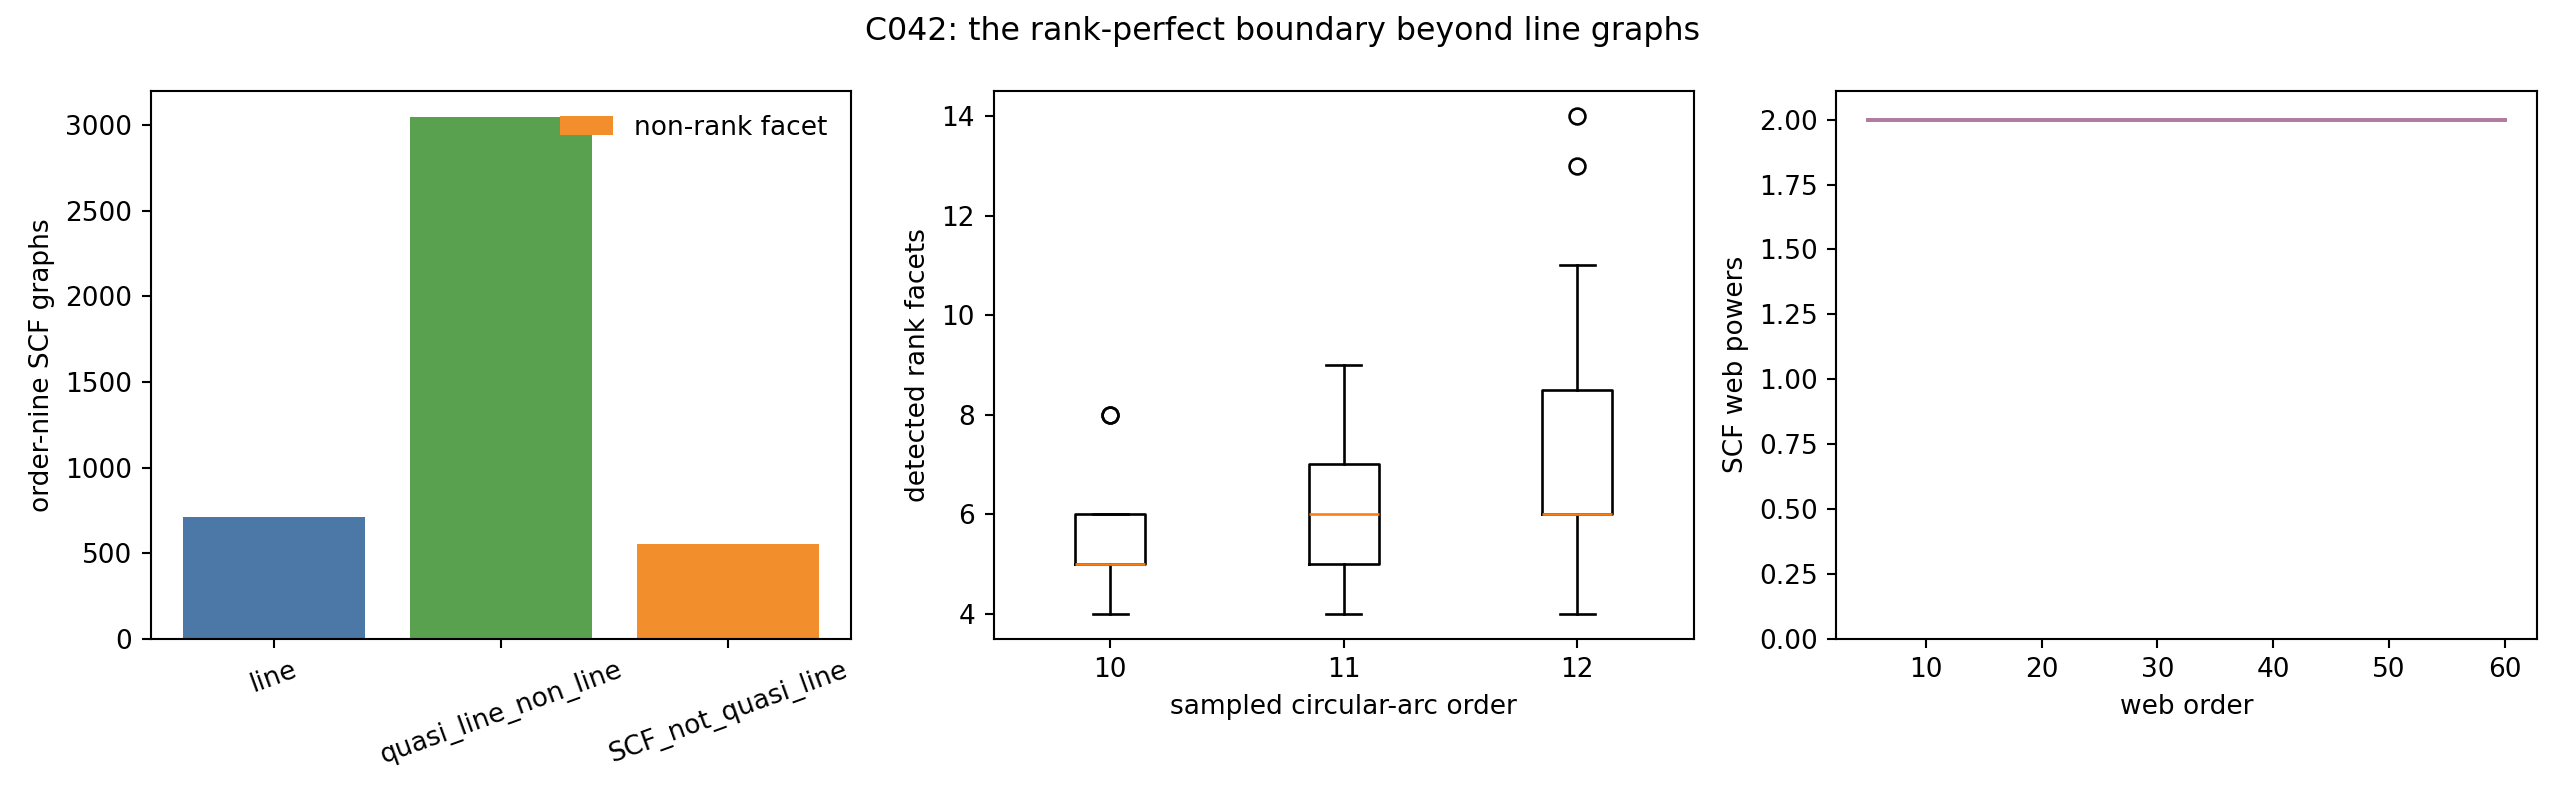
\includegraphics[width=\linewidth]{figures/c042_rank_perfect_boundary.png}
\caption{Rank-perfect boundary audit preceding the analytic closure. The order-nine panel is exhaustive for
the frozen SCF census; the larger proper circular-arc panel is a conditioned
seeded sample, and the web panel is an exact family sweep. The C043 proof no
longer depends on these finite observations.}
\label{fig:rank-perfect-boundary}
\end{figure}

The SCF hypothesis is essential. The unrestricted statement that all
quasi-line graphs are $\hbar$-perfect is false: the anti-heptagon is
quasi-line, has no simplicial clique, and is the smallest known
$\hbar$-imperfect graph~\cite{xu}. The theorem likewise makes no claim for
SCF graphs outside the quasi-line class.

\section{Baseline comparison and mechanism ablations}

The proof identifies a specific chain---skew contraction, squared entries,
and the complete matching polytope. We tested whether any named link is
dispensable. The benchmark contains every nonempty unlabeled root in the
NetworkX graph atlas through order seven. Each of the 1245 roots receives one
uniform and four seeded positive integer weight vectors, for 6225 weighted
instances. This is exhaustive over the small unweighted root types, but the
four nonuniform weights are stress cases rather than a probability model for
applications.

For each instance we compare the exact maximum-weight matching against three
linear relaxations on the same edge coordinates: degree inequalities only;
degree, root-triangle clique, and all simple odd-root-cycle inequalities; and
degree plus every odd-root-vertex-set inequality. In line-graph coordinates,
the second is the clique-and-odd-hole system used by the $h$-perfect route,
while the third is Edmonds' full matching polytope.

\begin{table}[H]
\centering
\caption{Relaxation value divided by exact maximum matching weight over 6225
weighted instances. ``Exact'' uses relative tolerance $2\times10^{-7}$.}
\label{tab:baselines}
\footnotesize
\begin{tabular}{lrrrrr}
\toprule
Baseline & Mean & Median & 95th pct. & Maximum & Exact \\
\midrule
Degree only & 1.0351 & 1.0000 & 1.1667 & 1.5000 & 66.89\% \\
Cliques + odd cycles & 1.0168 & 1.0000 & 1.1667 & 1.2500 & 84.69\% \\
All odd sets & 1.0000 & 1.0000 & 1.0000 & 1.0000 & 100.00\% \\
\bottomrule
\end{tabular}
\end{table}

Degree-only is strict on 2061 weighted cases from 797 roots; adding the
clique-and-odd-cycle constraints still leaves 953 strict cases from 555 roots.
The full odd-set system agrees with the discrete matching value in every
instance. The maximum degree gap is the uniform triangle, $3/2$ versus $1$.
The maximum second-baseline gap is $5/2$ versus $2$ on a five-vertex,
nine-edge root; the same $5/4$ ratio occurs for $K_5$. Figure~\ref{fig:gaps}
shows both the aggregate distribution and its dependence on root order.

\begin{figure}[t]
\centering
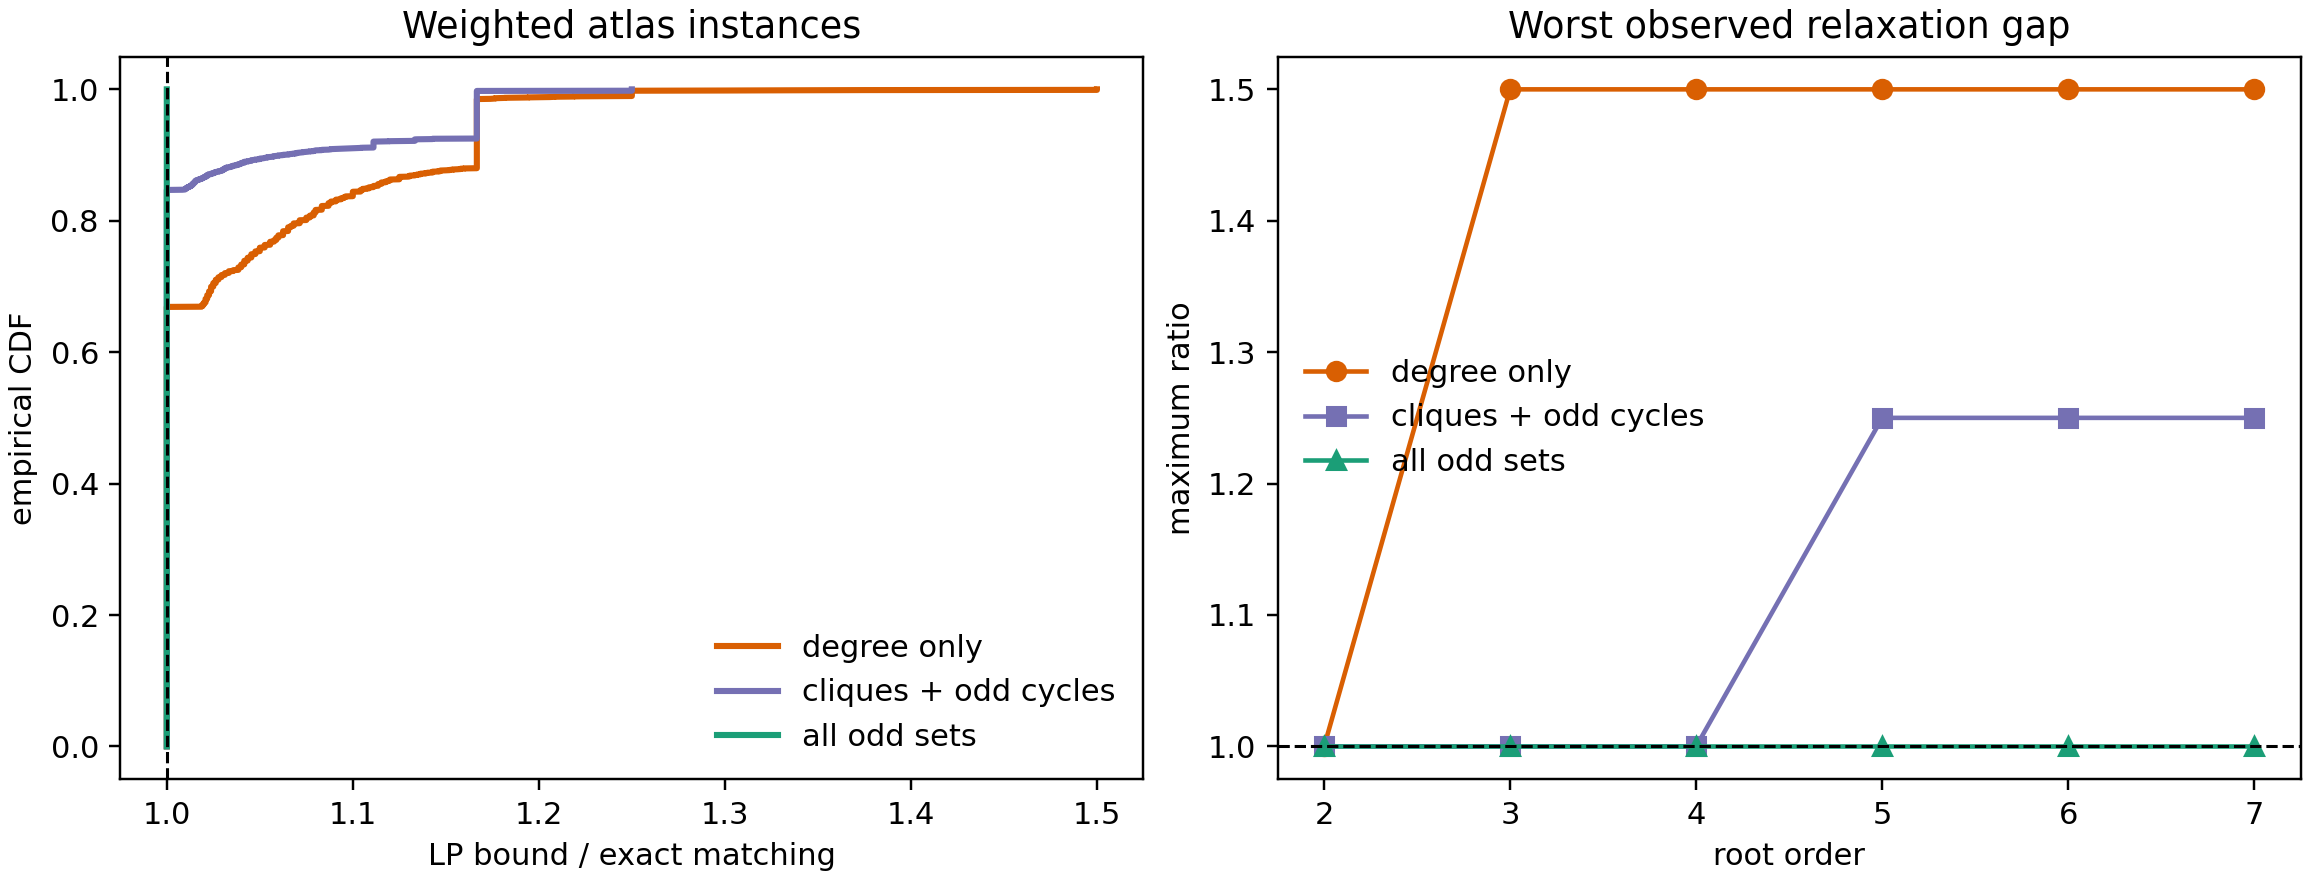
\includegraphics[width=\linewidth]{figures/c039_baseline_gaps.png}
\caption{Weaker relaxations systematically overestimate weighted matching.
The complete blossom system closes every tested gap. Percentages describe
this finite benchmark, not a population of quantum models.}
\label{fig:gaps}
\end{figure}

The bipartite subset is a positive control: all three descriptions are exact
on all 710 weighted cases. Among the 5515 nonbipartite cases, degree-only is
exact on 62.63\%, the clique-and-odd-cycle baseline on 82.72\%, and the full
polytope on 100\%. Thus the implementation recovers the classical bipartite
boundary before detecting the missing nonbipartite inequalities.

Controlled families separate the two kinds of odd constraint. With uniform
weights on an odd cycle $C_n$, the odd-cycle constraint repairs the
degree-only value $n/2$ to the matching value $(n-1)/2$. On an odd complete
root $K_n$, however, both weaker relaxations retain value $n/2$, exceeding the
matching value by $1/2$. We checked $n=5,7,9,11,13$. The complete-root blossom,
not another local cycle inequality, is the missing object.

Skewness is also necessary. On $K_3$, let $Q=I-(2/3)J$. This symmetric
Householder matrix has operator norm one and each off-diagonal square is
$4/9$. Every degree sum is only $8/9$, but the triangle odd-set sum is
$4/3>1$. A general contraction can therefore pass all degree tests and fail
the matching polytope. In contrast, the skew cross-product matrix generated
by $(1,1,1)/\sqrt3$ has norm one, edge squares $1/3$, and triangle sum exactly
one. The odd-dimensional rank loss used in Lemma~\ref{lem:contraction} is
precisely what disappears in the ablation.

Finally, the sharp constant should not be confused with typical saturation.
Across 4980 seeded Gaussian coefficient directions, the median theorem ratio
is $0.3992$, the 95th percentile is $0.7360$, and the maximum is one. After
excluding roots with fewer than three edges or matching value below two, the
corresponding values are $0.3968$, $0.7129$, and $0.9997$. By contrast, one
matching-supported construction for every root gives ratio exactly one in all
1245 cases. The theorem is an exact worst-case support function, not a claim
that generic Hamiltonians nearly saturate it. Figure~\ref{fig:ablations}
collects these controlled checks.

\begin{figure}[t]
\centering
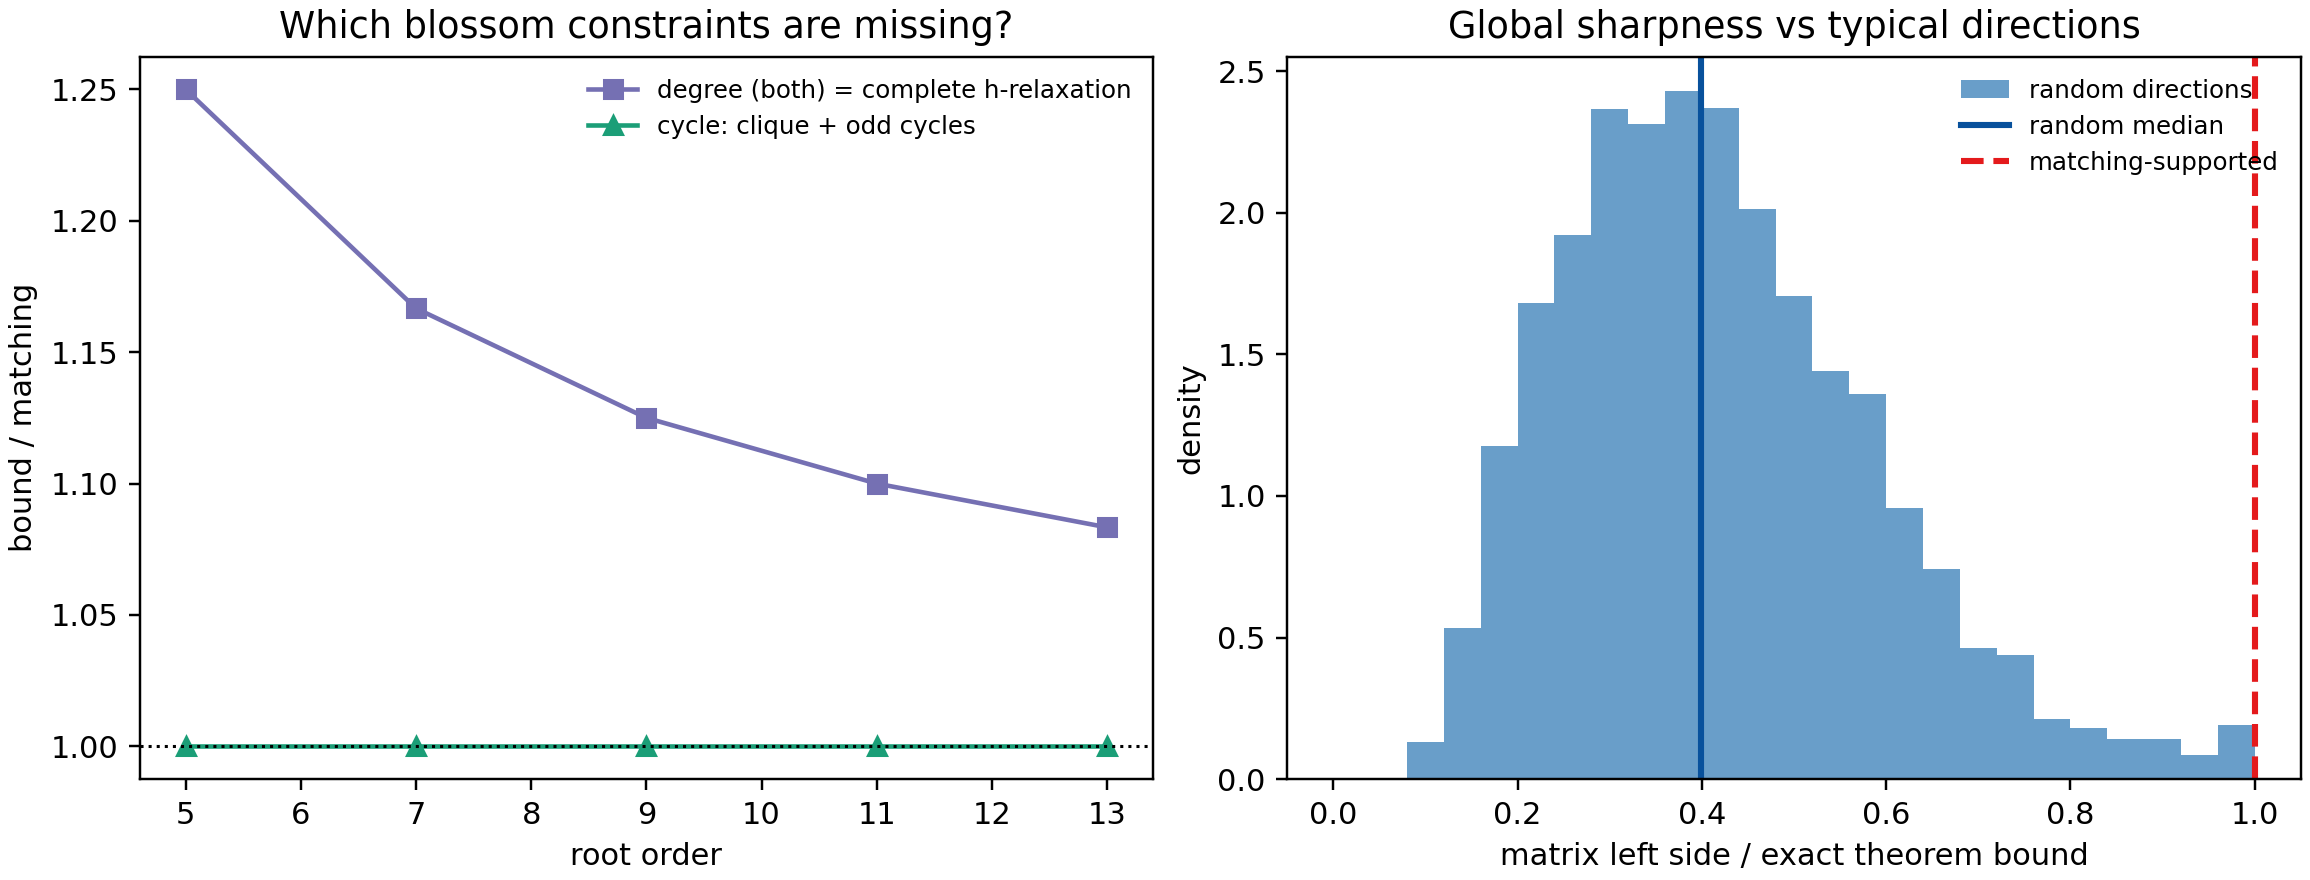
\includegraphics[width=\linewidth]{figures/c039_mechanism_ablations.png}
\caption{Mechanism ablations. Odd cycles repair cycle roots but not odd
complete roots; removing skewness violates the blossom constraint; random
directions are usually nonsaturating although equality is globally attainable.}
\label{fig:ablations}
\end{figure}

\section{Contribution hierarchy, priority boundary, and conclusion}

The paper has one headline result: for every finite root graph and every
nonnegative weight, the complete Pauli beta body of its line graph is the
classical matching polytope. Lemma~\ref{lem:contraction} is the mechanism, and
Theorem~\ref{thm:matrix} is its support-sensitive matrix form. The second
graph-polyhedral proof, the strict $L(K_{2k+1})$ separation, and the central
ablations are robustness checks and consequences of that result.

The simplicial claw-free quasi-line theorem is a secondary structural
extension. It establishes that the line-graph identity is not an isolated
coincidence, but it relies on the published quasi-line facet classification
and is not needed for Theorem~\ref{thm:main}. Keeping that dependency explicit
also makes the main theorem independently assessable if a referee asks for
the extension to be split off.

The closest prior literatures contain the ingredients separately. Beta
numbers and representation invariance are due to Xu et al.~\cite{xu,xuprx};
line-graph Majorana solvability is due to Chapman and
Flammia~\cite{cf}; and Edmonds supplies the matching polytope and weighted
oracle~\cite{edmonds}. Skew-energy and trace-norm work relates spectral
quantities to matching, rank, or degree~\cite{tianwong,zhoutrace}, while
McNulty studies a different line-graph invariant, measurement
incompatibility~\cite{mcnulty}. The priority-sensitive conjunction here is
the all-weight beta/matching identity, the generation of every blossom
inequality by odd skew contractions, and the arbitrary-entry weighted matrix
form. A source-by-source C045 audit found no exact statement of that
conjunction. Negative search cannot establish priority, so we make no
``first'' claim and retain external refereeing as the independent check.

In summary, odd principal submatrices of a skew contraction lose one rank.
That fact supplies every blossom inequality and converts an exact quantum
uncertainty problem into maximum-weight matching. The result is analytic,
arbitrary-size, and all-weight; it is not a hardware, speedup, or new
matching-algorithm claim. The appendices report the broader computational
falsification, proof-hardening ledger, and expanded source boundary.

\appendix

\section{Scaling, density, and weak coupling}

The atlas is exhaustive but small. A separate preregistered campaign samples
180 sparse roots at orders $10,14,18,22,26,30$: six replicates from each of
five generators, with uniform, integer, lognormal, and Pareto edge weights.
For each of 720 weighted instances we compare a nested hierarchy: degree
constraints, all line-graph clique constraints, and every simple odd-root-cycle
constraint through lengths five, seven, and nine. The reference value is exact
maximum-weight matching. Forty cases at orders 10 and 14 also enumerate every
odd vertex set; their full blossom LPs all equal matching.

\begin{table}[H]
\centering
\caption{Scaled sparse ensemble. Ratios are LP value divided by exact matching.
The odd-cycle rows are truncated at the displayed length.}
\label{tab:scaled}
\small
\begin{tabular}{lrrrr}
\toprule
Baseline & Mean & 95th pct. & Maximum & Exact \\
\midrule
Degree only & 1.007353 & 1.045550 & 1.500000 & 77.22\% \\
All cliques & 1.002541 & 1.013284 & 1.166667 & 91.67\% \\
Odd cycles $\leq5$ & 1.002156 & 1.008641 & 1.166667 & 93.47\% \\
Odd cycles $\leq7$ & 1.002068 & 1.005697 & 1.166667 & 93.89\% \\
Odd cycles $\leq9$ & 1.002041 & 1.005697 & 1.166667 & 93.89\% \\
\bottomrule
\end{tabular}
\end{table}

Figure~\ref{fig:scaled-random} shows that local constraints are numerically
close on most sampled sparse graphs, especially with heterogeneous weights,
but do not converge to universal exactness. Under the odd-through-nine
baseline, exact fractions are 87.22\%, 93.33\%, 99.44\%, and 95.56\% for
uniform, integer, lognormal, and Pareto weights. These values describe the
frozen generators and seeds, not an application distribution.

\begin{figure}[t]
\centering
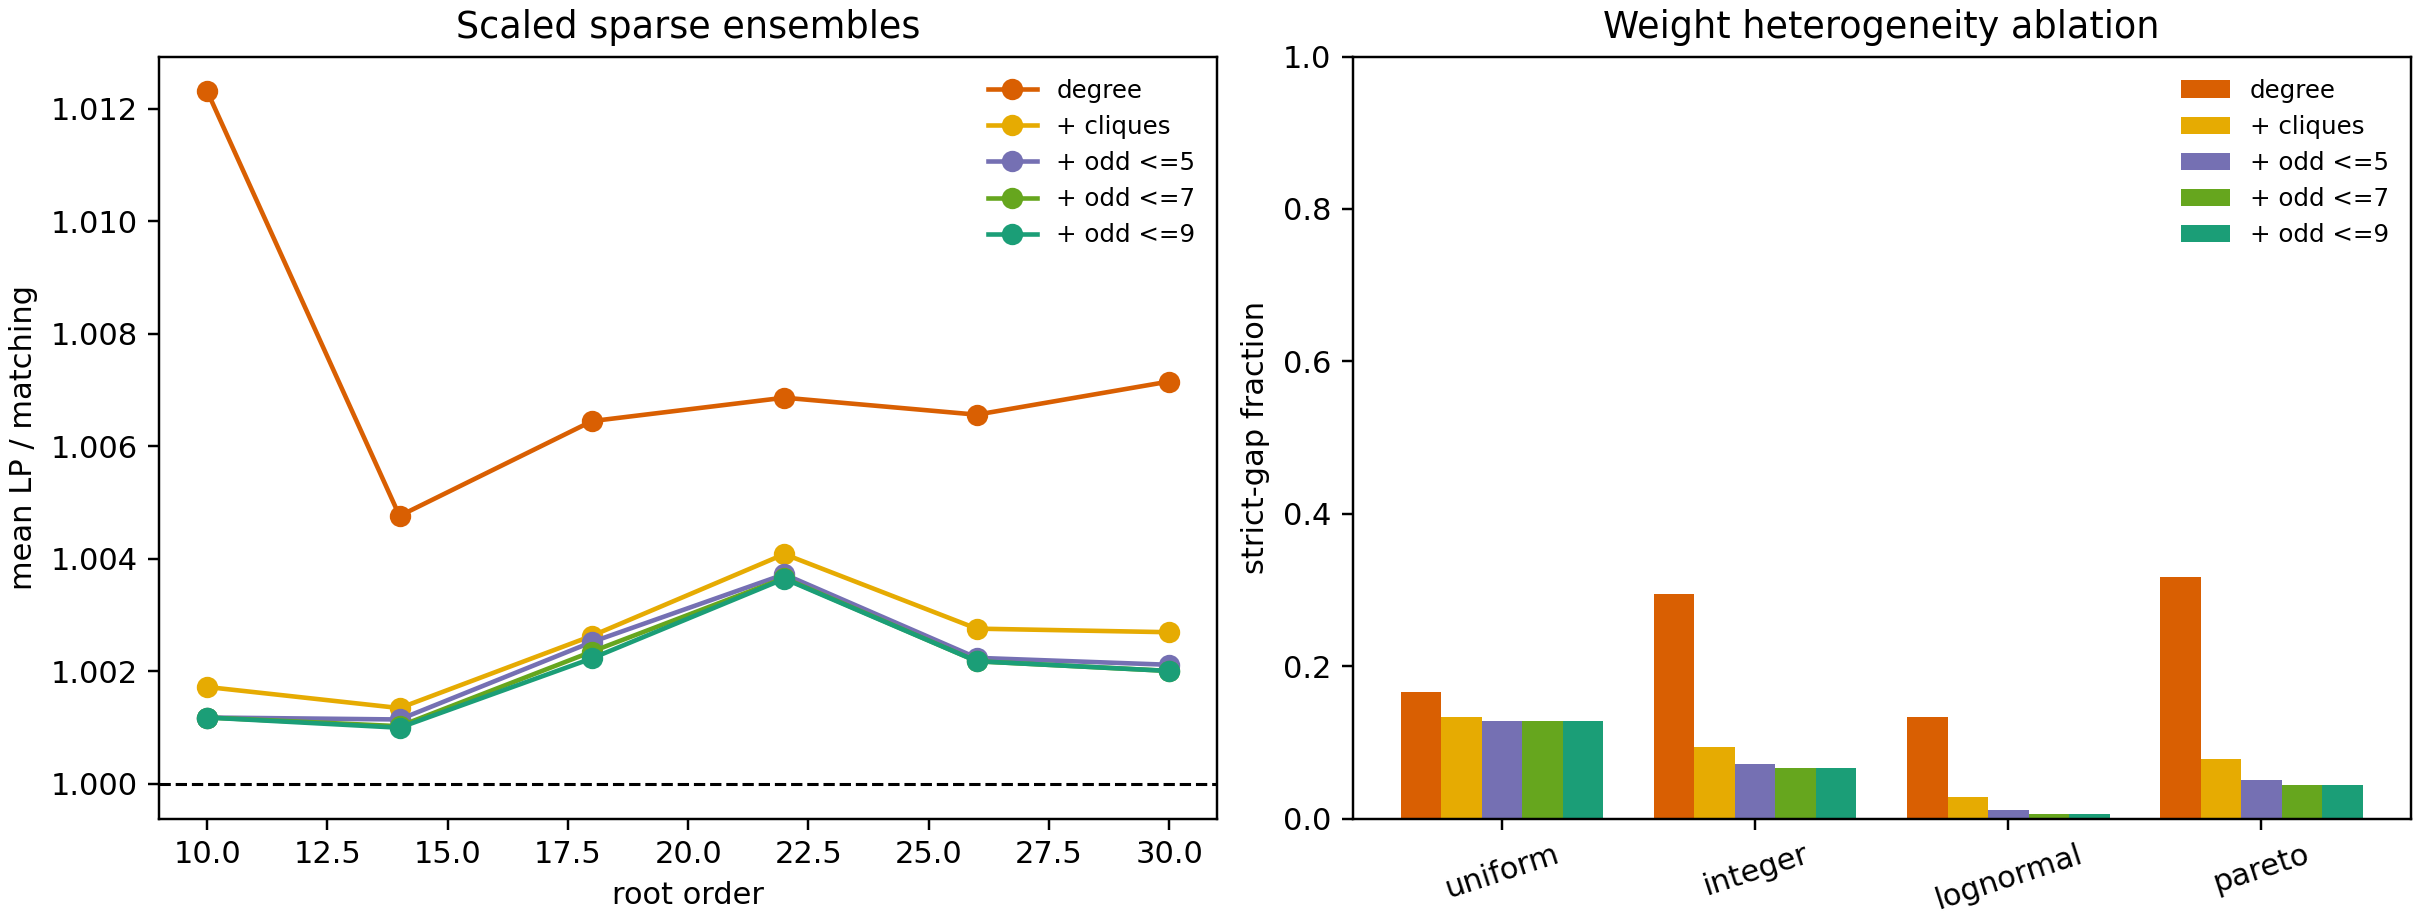
\includegraphics[width=\linewidth]{figures/c040_scaled_random_ablations.png}
\caption{Scaling and weight ablations on 720 weighted sparse instances. Local
constraints usually make the remaining gap small, but exactness depends on
the graph and weight ensemble.}
\label{fig:scaled-random}
\end{figure}

Controlled direct sums prevent a misleading ``typical equals sufficient''
interpretation. Disjoint $K_3,C_5,C_7,C_9,C_{11}$ components retain ratios
$3/2,5/4,7/6,9/8,11/10$ until the corresponding missing local constraint is
added. More importantly, disjoint $K_5$ components retain ratio $5/4$ after
all odd cycles through nine, although every simple cycle within a component is
already covered. The missing inequality is the full five-vertex blossom.
Orders reach 132, so the gap is not a vanishing finite-size effect.

For 540 Gaussian matrix directions on the scaled roots, the median theorem
ratio is $0.3315$, the 95th percentile is $0.4982$, and the maximum is
$0.7418$; 180 matching-supported controls all attain one. Removing skewness
also scales: block-diagonal copies of the symmetric Householder counterexample
retain violation ratio $4/3$ through order 96. Figure~\ref{fig:structured}
summarizes both controls.

\begin{figure}[t]
\centering
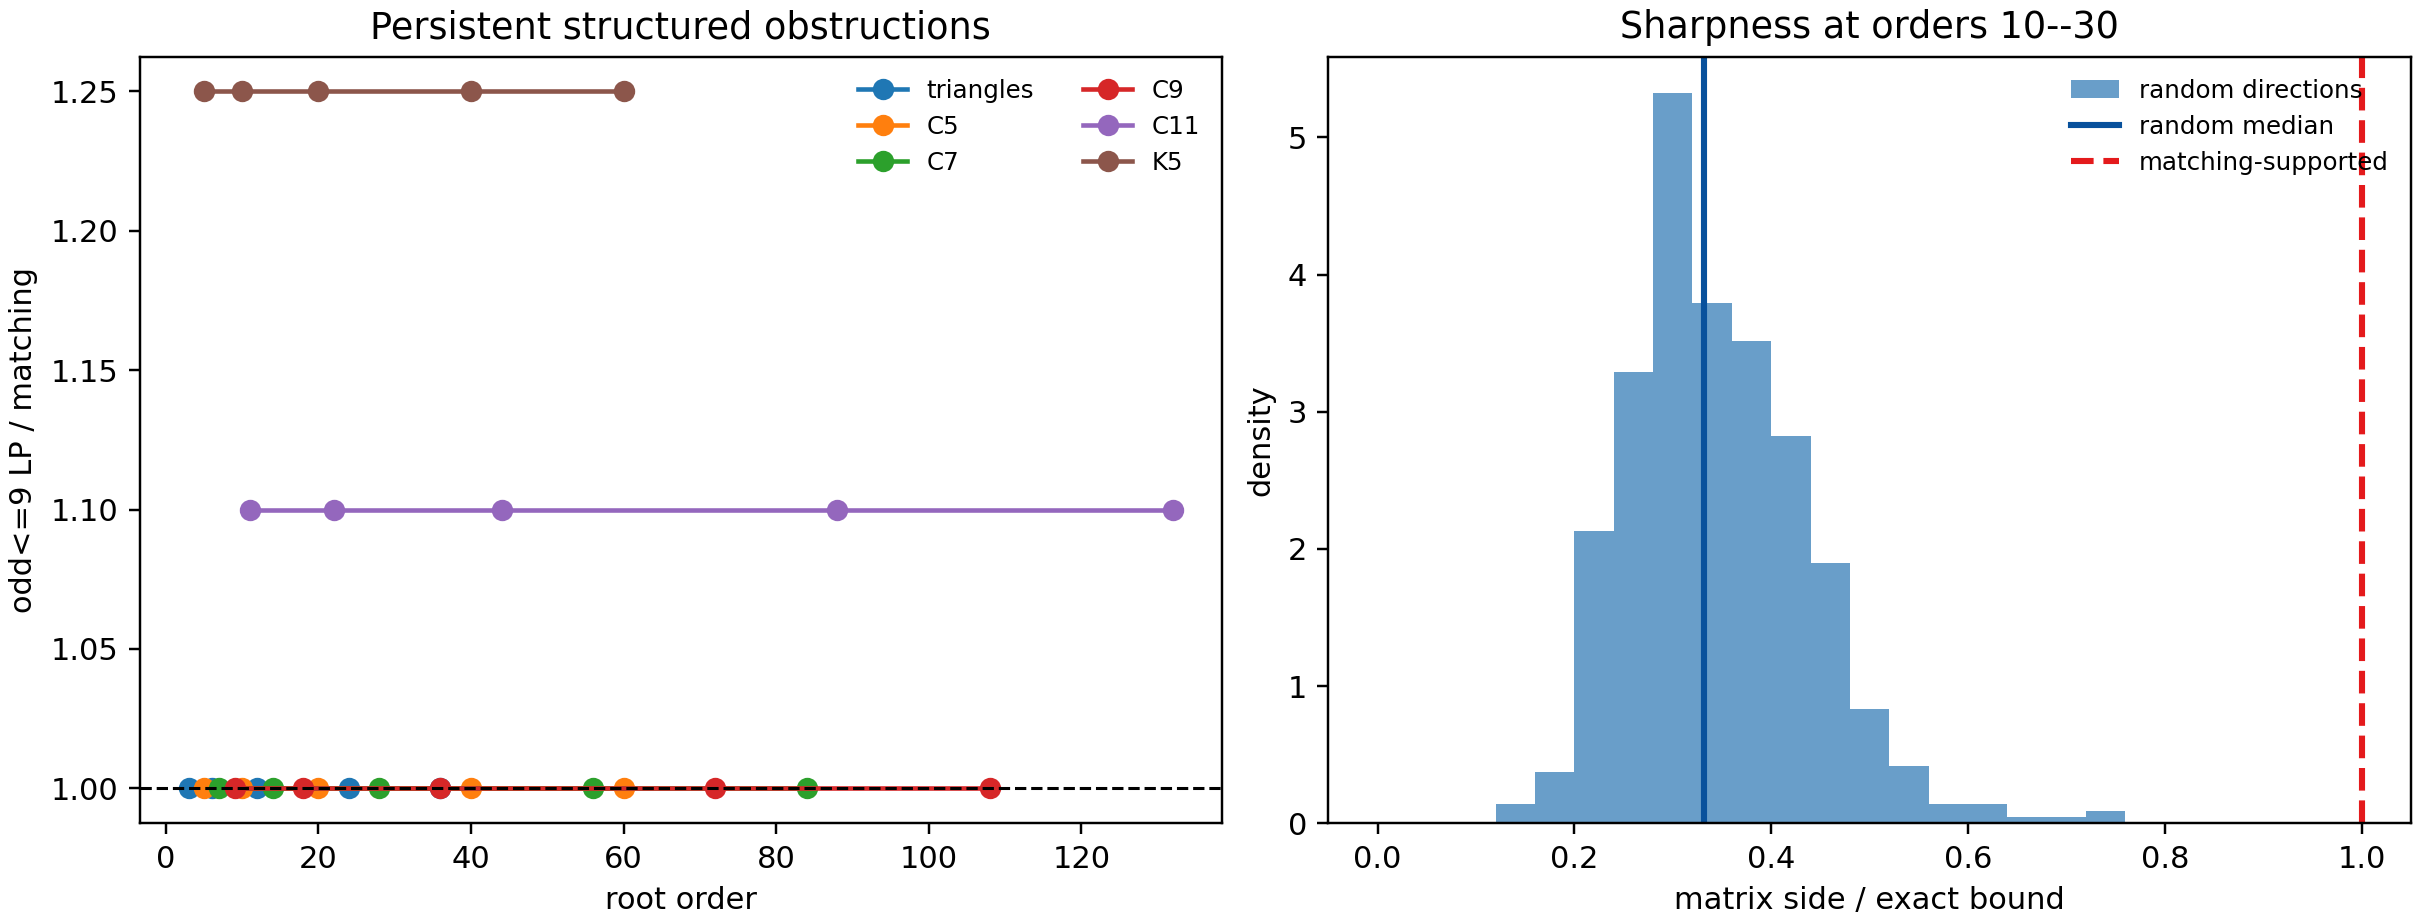
\includegraphics[width=\linewidth]{figures/c040_structured_and_tightness.png}
\caption{Left: local obstructions persist under direct sums. Right: generic
Gaussian directions are far from equality while matching-supported directions
remain exactly sharp.}
\label{fig:structured}
\end{figure}

A final density stress uses 45 Erdos--Renyi roots at orders 20, 30, and 40,
expected degrees two through six, and two weight regimes. Odd-through-nine is
strict in 5 of 90 weighted cases, with maximum ratio $29/28$. One graph already
contains 384,484 enumerated odd cycles through length nine; the complete run
takes 393.7 seconds. Thus explicit local-cycle enumeration can become large
even when its remaining value gap is small.

To test robustness beyond disconnected unions, even numbers of $K_5$ blocks
are joined in a ring by weak weighted bridges. With $b$ blocks and bridge
weight $\varepsilon$, the observed local optimum is $2.5b$ and matching is
$2b+\varepsilon b/2$, giving ratio
\[
 \frac{2.5}{2+\varepsilon/2}.
\]
It is $1.2195$ at $\varepsilon=0.1$, $1.1111$ at $\varepsilon=0.5$, and closes
only at unit bridge weight, identically for 2, 4, 8, and 16 blocks (up to 80
vertices). Figure~\ref{fig:density} separates this planted mechanism from the
nonmonotone random density sweep.

\begin{figure}[t]
\centering
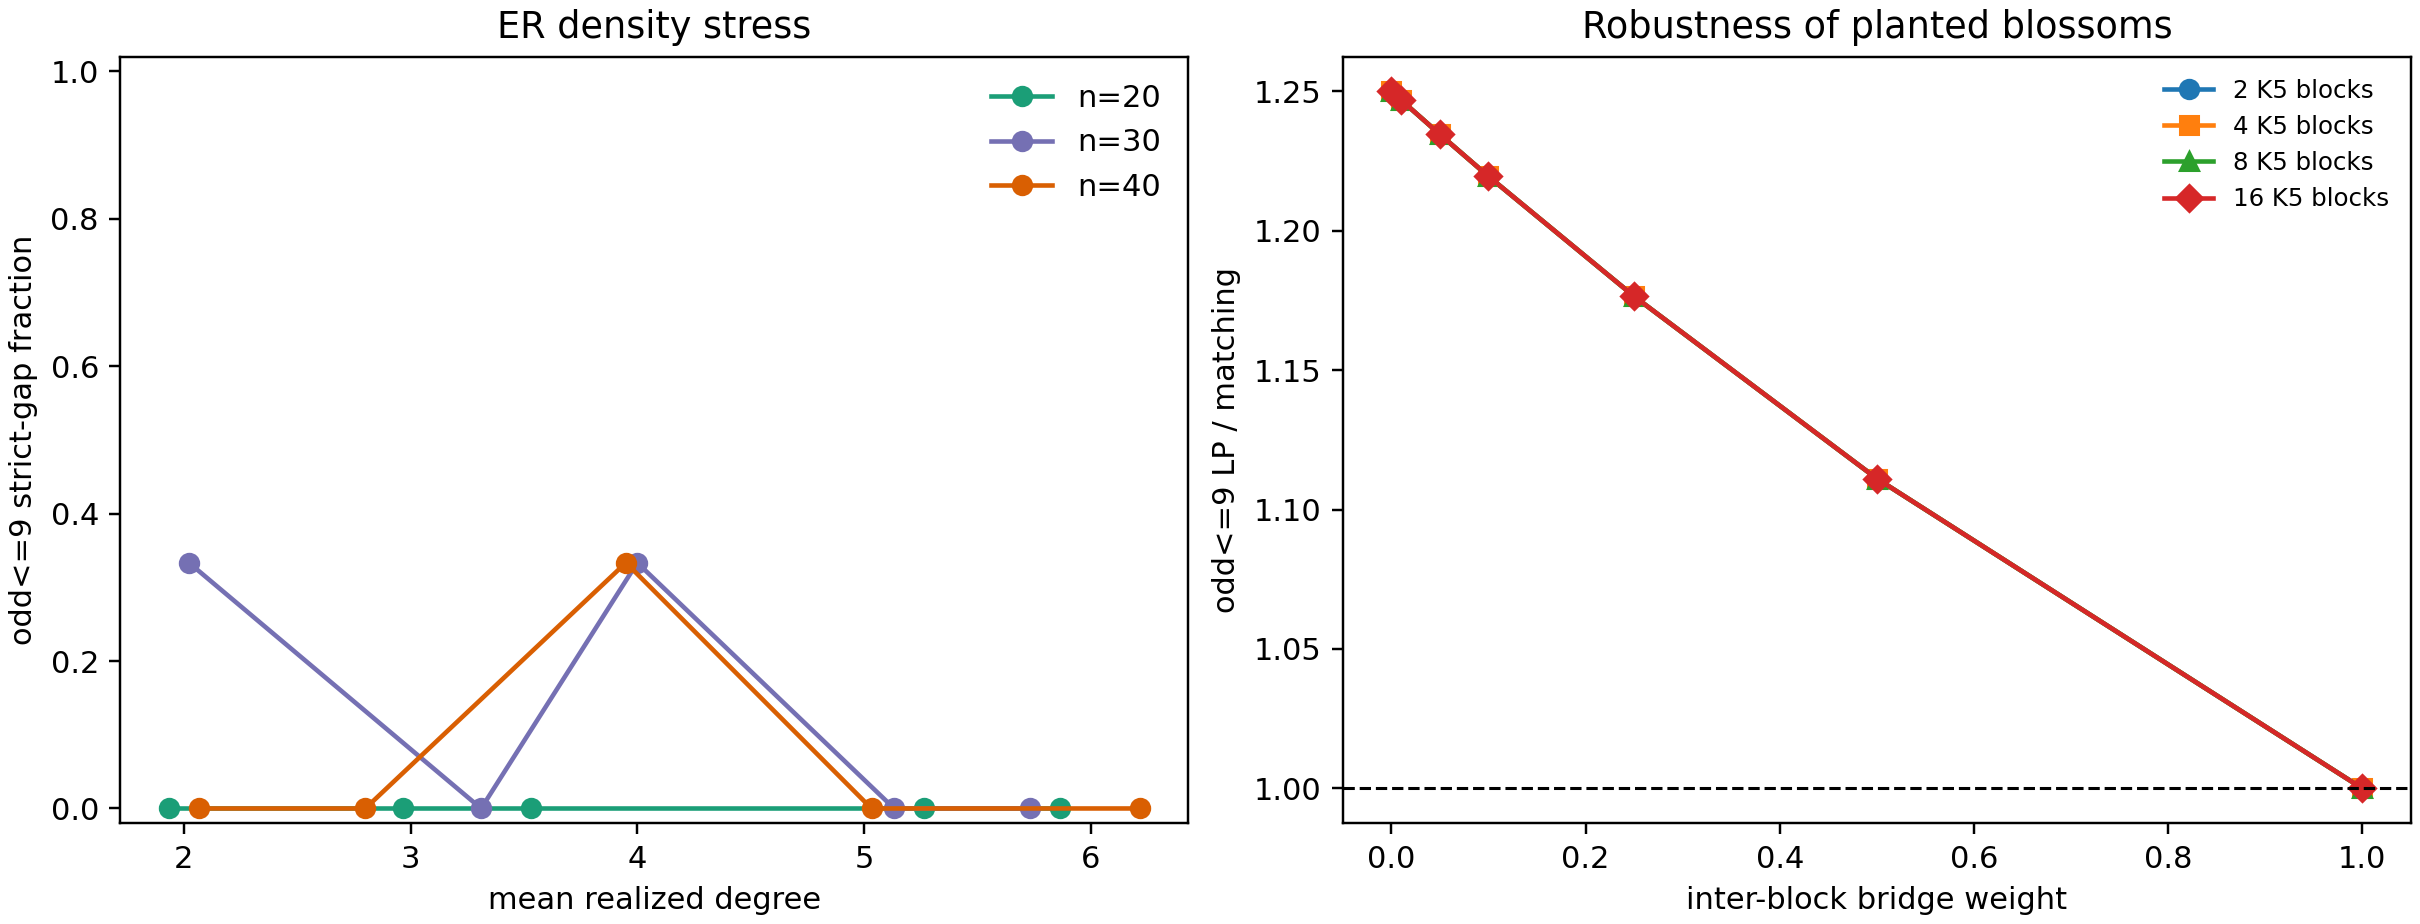
\includegraphics[width=\linewidth]{figures/c041_density_coupling_stress.png}
\caption{Density and weak-coupling stress. Random exactness is nonmonotone,
whereas planted blossom gaps survive connectivity and weak bridges with a
size-independent curve.}
\label{fig:density}
\end{figure}

\section{Computational falsification and reproducibility}

The proof is arbitrary-size and does not depend on enumeration. We nevertheless
implemented a stress audit designed to expose normalization, orientation, and
odd-set errors. It evaluates every nonempty graph in the NetworkX graph atlas,
giving 1245 root graphs of order at most seven. For random positive weights and
supported skew matrices, the code independently computes maximum-weight
matching, the nuclear-norm expression, a polar dual optimizer, all degree and
odd-set residuals, and the theorem ratio.

The largest observed ratio to the proved bound is
$1.0000000000000002$. The maximum polar-pairing discrepancy is
$3.20\times10^{-14}$; maximum degree and odd-set excesses are
$1.33\times10^{-15}$ and $2.22\times10^{-15}$. In 47 small-root cases a dense
Jordan--Wigner construction directly checks~\eqref{eq:maj-norm}; its maximum
error is $7.11\times10^{-15}$. Exact rational records for $K_5,K_7,K_9$
check the strict separation. A standard-library verifier checks the frozen
summary and source hash, while five tests deliberately corrupt the gap, scope,
hash, or norm data and require rejection.

The baseline-and-ablation run is independently frozen in a second JSON file,
three CSV tables, and two figures. Its verifier recomputes every aggregate,
checks all 6225 full-polytope equalities, proves the Householder counterexample
with rational arithmetic, checks the controlled-family formulas, and verifies
SHA-256 hashes of all five derived artifacts. Five additional corruption tests
require rejection of altered ratios, counterexample entries, hashes, or scope
flags.

The two scaled records add 225 sampled roots, 810 weighted random instances, 58
structured or coupling rows, ten hashed tables or figures, two independent
standard-library verifiers, and eleven corruption tests. Their scope fields
explicitly distinguish seeded ensembles, truncated odd-cycle systems, and
controlled constructions from exhaustive or application-level claims.

The C042 record adds an exhaustive reclassification of 4308 order-nine SCF
graphs, 868 web graphs, and 60 conditioned proper circular-arc stress graphs.
Its independent verifier reconstructs the graph classes, strict witness, and
exact rank-facet certificates. Six tests include five intentional corruptions.

The C043 record independently checks 4308 deterministic induced deletions,
6162 circulant parameter pairs through order 160, all 18,149 cliques in the
small circulants through order 18, one exact published nonrank-web positive
control, and 250 exact clique-family stress graphs. The small exact sweep
explicitly includes the nonlocal clique $\{0,3,6\}$ in $C(9,4)$ that falsifies
the tempting local-cliques-only proof. Its standard-library verifier
reconstructs the circulant witnesses and the positive-control facet; five
mutation tests must reject corrupted records.

C044 removes the only geometric proof sketch from the new theorem. Its
left/right sumset argument is fully contained in Lemma~\ref{lem:circulant-obstruction}.
The corresponding audit checks all 38,772 one-vertex deletions of the frozen
SCF census, 1,027,351 admissible algebra rows through order 160, 4,194,302
deficit subsets, and all 3,803,174 cliques of every $C(n,p)$ through order 30.
No simplicial clique occurs for $p\geq3$. A separate standard-library verifier
recomputes the algebra and sumset counts, checks all frozen hashes, and is
protected by five mutation tests.

C046 is a claim-level mock-referee audit of the headline proof. It separates
the realization-dependent raw joint range from the invariant beta body,
checks the compact-convex support-function step, and makes the odd-order
Clifford normalization explicit. Its verifier rejects a missing body identity,
the old representation quantifier, an altered report, and false review-status
flags. This is an internal adversarial check, not external peer review.

From the repository root:
\begin{quote}\small\ttfamily\raggedright
python experiments/pauli\_fourth\_moment\_phase0/\\
\hspace*{1em}run\_c038\_line\_graph\_hbar.py\par
python -S experiments/pauli\_fourth\_moment\_phase0/\\
\hspace*{1em}verify\_c038\_line\_graph\_hbar.py\par
python -m unittest discover -s\\
\hspace*{1em}experiments/pauli\_fourth\_moment\_phase0\\
\hspace*{1em}-p test\_c038\_line\_graph\_hbar.py -v
\medskip\par
python experiments/pauli\_fourth\_moment\_phase0/\\
\hspace*{1em}run\_c039\_central\_ablations.py --overwrite\par
python -S experiments/pauli\_fourth\_moment\_phase0/\\
\hspace*{1em}verify\_c039\_central\_ablations.py\par
python -m unittest discover -s\\
\hspace*{1em}experiments/pauli\_fourth\_moment\_phase0\\
\hspace*{1em}-p test\_c039\_central\_ablations.py -v
\medskip\par
python experiments/pauli\_fourth\_moment\_phase0/\\
\hspace*{1em}run\_c040\_scaled\_ablations.py --overwrite\par
python -S experiments/pauli\_fourth\_moment\_phase0/\\
\hspace*{1em}verify\_c040\_scaled\_ablations.py\par
python experiments/pauli\_fourth\_moment\_phase0/\\
\hspace*{1em}run\_c041\_density\_coupling\_stress.py --overwrite\par
python -S experiments/pauli\_fourth\_moment\_phase0/\\
\hspace*{1em}verify\_c041\_density\_coupling\_stress.py
\medskip\par
python experiments/pauli\_fourth\_moment\_phase0/\\
\hspace*{1em}run\_c042\_rank\_perfect\_boundary.py\par
python -S experiments/pauli\_fourth\_moment\_phase0/\\
\hspace*{1em}verify\_c042\_rank\_perfect\_boundary.py
\medskip\par
python experiments/pauli\_fourth\_moment\_phase0/\\
\hspace*{1em}run\_c043\_quasiline\_scf\_falsification.py --overwrite\par
python -S experiments/pauli\_fourth\_moment\_phase0/\\
\hspace*{1em}verify\_c043\_quasiline\_scf\_theorem.py
\medskip\par
python experiments/pauli\_fourth\_moment\_phase0/\\
\hspace*{1em}run\_c044\_proof\_hardening.py --overwrite\par
python -S experiments/pauli\_fourth\_moment\_phase0/\\
\hspace*{1em}verify\_c044\_proof\_hardening.py
\medskip\par
python -S experiments/pauli\_fourth\_moment\_phase0/\\
\hspace*{1em}verify\_c046\_mock\_referee\_body\_audit.py
\end{quote}
The wrapped paths are single commands. Numerical agreement is falsification
support, not the proof of Theorem~\ref{thm:main}.

\section{Expanded relation to prior work and claim boundary}

Chapman and Flammia identify line-graph frustration structures as the free
fermion setting for quadratic Majorana Hamiltonians~\cite{cf}. Chapman,
Elman, and Mann develop the wider simplicial claw-free framework~\cite{cem}.
Xu et al.~define weighted beta numbers and $\hbar$-perfection and establish
other sufficient graph classes~\cite{xu}; their accessible manuscript does
not state the all-line-graph weighted matching equality used here. Oriolo and
Eisenbrand et al.~supply the classical semi-line and quasi-line polyhedral
boundary~\cite{oriolo,eosv}. Oriolo and Stauffer's later clique-circulant
facet theorem~\cite{oriolostauffer2022} is the structural input to
Theorem~\ref{thm:scf-quasiline}.

The graphs $L(K_{2k+1})$ already appear in magic-state simulation via
Jordan--Wigner transformations~\cite{zurel}; the separating graphs themselves
are not new. McNulty studies measurement incompatibility on line graphs using
skew-energy bounds~\cite{mcnulty}. Classical skew-energy inequalities related
to matching are studied by Tian and Wong~\cite{tianwong}. The uniform shadow
of~\eqref{eq:matrix} is therefore close to known rank and skew-energy bounds.
Our priority-sensitive claim is the exact all-weight Pauli beta/matching
identity, its complete matching-polytope mechanism, and the sharp weighted
matrix form. The underlying ingredients -- Edmonds' theorem, nuclear duality,
Majorana normal form, and line-graph solvability -- are not claimed new.

The repository contains a source-by-source adversarial audit with explicit
overlap and falsification criteria. This supports careful positioning but
cannot exclude differently worded or inaccessible prior results. Journal
referees remain the independent priority check when no pre-submission expert
is available.

\section{Extended discussion and scope}

Odd principal submatrices of a skew contraction lose one rank. That elementary
fact generates every blossom inequality and turns the quantum optimization on
a line graph into the classical matching polytope. Consequently all finite
line graphs are $\hbar$-perfect for arbitrary nonnegative weights, and the
associated skew-matrix inequality is sharp. The infinite family
$L(K_{2k+1})$ shows that this mechanism is genuinely broader than the known
$h$-perfect sufficient route.

The ablations sharpen that interpretation. Degree constraints alone explain
the entire bipartite control but fail broadly outside it. Adding every clique
and odd-cycle inequality reduces rather than eliminates the gap, while full
odd-set constraints eliminate it. Removing skewness breaks the key conclusion
on the smallest possible odd root. These are finite tests of the proof's
named ingredients, not empirical substitutes for the theorem.

Scaling clarifies the practical boundary. Local constraints are often nearly
exact on seeded sparse ensembles, but constant gaps persist on direct sums and
under weak coupling. Explicitly enumerating short odd cycles can require
hundreds of thousands of rows by order 40, while the complete mathematical
object remains maximum-weight matching rather than an ever longer list of
local repairs.

The rank-perfect SCF bridge and the clique-circulant obstruction show that the
line-graph mechanism is not the only analytic route. Exact Pauli uncertainty
extends to every SCF quasi-line graph, including a certified graph that is
neither line nor $h$-perfect. The unrestricted SCF and unrestricted
quasi-line statements remain outside the theorem.

The result concerns exact uncertainty values, not quantum advantage or hardware
performance. The next scientific tests are independent refereeing and a wider
bibliographic priority search; adding more random instances would not strengthen
the analytic theorem.

\section*{Data and code availability}

Source, frozen records, verifier, and tests are available in the
\href{https://github.com/YaroslavPelekhov/Quantum/tree/research/c038-line-graph-hbar}{public C038 GitHub branch}.
The repository index identifies the theorem note, priority audit, generator,
frozen JSON, independent verifiers, and corruption-controlled tests. Every
reported numerical constant is read from nine frozen JSON records by the
manuscript checker. They include graph identifiers, generator seeds, weight
regimes, relaxation values, aggregate summaries, explicit scope flags, and
hashes for all derived tables and figures.

\section*{Declarations}

No external funding, competing-interest, authorship, affiliation, or
AI-assistance declaration is made in this anonymous working version. These
fields must be completed truthfully by the author before submission. No QPU
data are used in the theorem or its verification.

\begin{thebibliography}{99}
\small
\bibitem{edmonds}
J. Edmonds, \emph{Maximum matching and a polyhedron with 0,1-vertices},
Journal of Research of the National Bureau of Standards B 69B, 125--130
(1965). \url{https://doi.org/10.6028/jres.069B.013}.

\bibitem{cf}
A. Chapman and S. T. Flammia,
\emph{Characterization of solvable spin models via graph invariants},
Quantum 4, 278 (2020).
\url{https://doi.org/10.22331/q-2020-06-04-278}.

\bibitem{cem}
A. Chapman, S. J. Elman, and R. L. Mann,
\emph{A Unified Graph-Theoretic Framework for Free-Fermion Solvability},
arXiv:2305.15625 (2023).
\url{https://arxiv.org/abs/2305.15625}.

\bibitem{xu}
Z.-P. Xu, J. Wang, Q. Ye, G. Ko\ss mann, R. Schwonnek, and A. Winter,
\emph{Simultaneous variances of Pauli strings, weighted independence numbers,
and a new kind of perfection of graphs}, arXiv:2511.13531 (2025).
\url{https://arxiv.org/abs/2511.13531}.

\bibitem{xuprx}
Z.-P. Xu, R. Schwonnek, and A. Winter,
\emph{Bounding the joint numerical range of Pauli strings by graph
parameters}, PRX Quantum 5, 020318 (2024).
\url{https://doi.org/10.1103/PRXQuantum.5.020318}.

\bibitem{oriolo}
G. Oriolo, \emph{Clique family inequalities for the stable set polytope of
quasi-line graphs}, Discrete Applied Mathematics 132, 185--201 (2003).
\url{https://doi.org/10.1016/S0166-218X(03)00400-1}.

\bibitem{eosv}
F. Eisenbrand, G. Oriolo, G. Stauffer, and P. Ventura,
\emph{The stable set polytope of quasi-line graphs}, Combinatorica 28,
45--67 (2008). \url{https://doi.org/10.1007/s00493-008-2169-1}.

\bibitem{oriolostauffer2022}
G. Oriolo and G. Stauffer,
\emph{On the facets of stable set polytopes of circular interval graphs},
Annals of Operations Research 315, 1551--1573 (2022).
\url{https://doi.org/10.1007/s10479-021-04449-7}.

\bibitem{csss}
M. Chudnovsky, A. Scott, P. Seymour, and S. Spirkl,
\emph{A note on simplicial cliques},
Discrete Mathematics 344, 112470 (2021).
\url{https://doi.org/10.1016/j.disc.2021.112470}.

\bibitem{zurel}
M. Zurel, L. Z. Cohen, and R. Raussendorf,
\emph{Simulation of quantum computation with magic states via Jordan--Wigner
transformations}, Physical Review A 112, 042602 (2025).
\url{https://doi.org/10.1103/ng4l-96kd}.

\bibitem{mcnulty}
D. McNulty, \emph{A Graph-Theoretic Approach to Quantum Measurement
Incompatibility}, arXiv:2511.15954 (2025).
\url{https://arxiv.org/abs/2511.15954}.

\bibitem{tianwong}
F. Tian and D. Wong, \emph{Relation between the skew energy of an oriented
graph and its matching number}, Discrete Applied Mathematics 222, 179--184
(2017). \url{https://doi.org/10.1016/j.dam.2017.01.004}.

\bibitem{zhoutrace}
Q. Zhou, F. Xu, Y. Zhang, and D. Wong,
\emph{Relation between the trace norm of an oriented graph and its rank},
Linear Algebra and its Applications 675, 204--218 (2023).
\url{https://doi.org/10.1016/j.laa.2023.06.023}.
\end{thebibliography}

\end{document}
